%===========================================================================
\chapter{Logic Synthesis and FPGA Implementation}\label{ch:synth}
%===========================================================================

The RTL was synthesised with the open-source \textbf{Yosys 0.70} synthesis
suite~\cite{yosys} and placed and routed with \textbf{nextpnr-ecp5}~\cite{nextpnr}.
Four flows were used (scripts in Appendix~\ref{app:synth}). The first flow
produces the RTL schematics: Yosys elaborates the design, and
netlistsvg~\cite{netlistsvg} draws the resulting netlist. The second flow is
generic (ASIC-style) gate-level synthesis, in which technology mapping with
ABC targets 2-input gates and D flip-flops, applied both to the MAC unit and
to the complete processor. The third flow is FPGA implementation on a Lattice
ECP5 LFE5U-85F (\code{synth\_ecp5} + nextpnr place \& route, speed grade~6),
carried out for the MAC unit with the Booth multiplier, for the MAC unit with
hard DSP multipliers as a comparison, and for the complete RV32IM core with
the MAC unit. The fourth flow is post-synthesis gate-level simulation of the
synthesised netlist.

\section{RTL schematics generated by Yosys}
Figure~\ref{fig:sch_booth} shows the radix-4 Booth multiplier as Yosys
elaborates it. A small instance ($W=6$) is used so that the structure stays
readable. Each of the three 3-bit groups of $B$ is decoded by \code{\$eq}
comparators that drive a Booth-recoding multiplexer (\code{\$pmux}) choosing
$0,\pm A,\pm 2A$. Yosys then merged the weighted partial-product additions
into multiply-accumulate (\code{\$macc}) and adder (\code{\$alu}) cells,
exactly as described in Table~\ref{tab:booth}. Figure~\ref{fig:sch_booth_g}
shows the same circuit after technology mapping: 216 two-input gates.
Figure~\ref{fig:sch_mac} shows the complete \code{mac\_unit}: the Booth
multiplier appears as one block, surrounded by the decoder, the stage-1 and
stage-2 registers (\code{\$dff}/\code{\$sdff}), the 65-bit adder and
subtractor, the saturation comparators and the result multiplexers.

\begin{figure}[H]
  \centering
  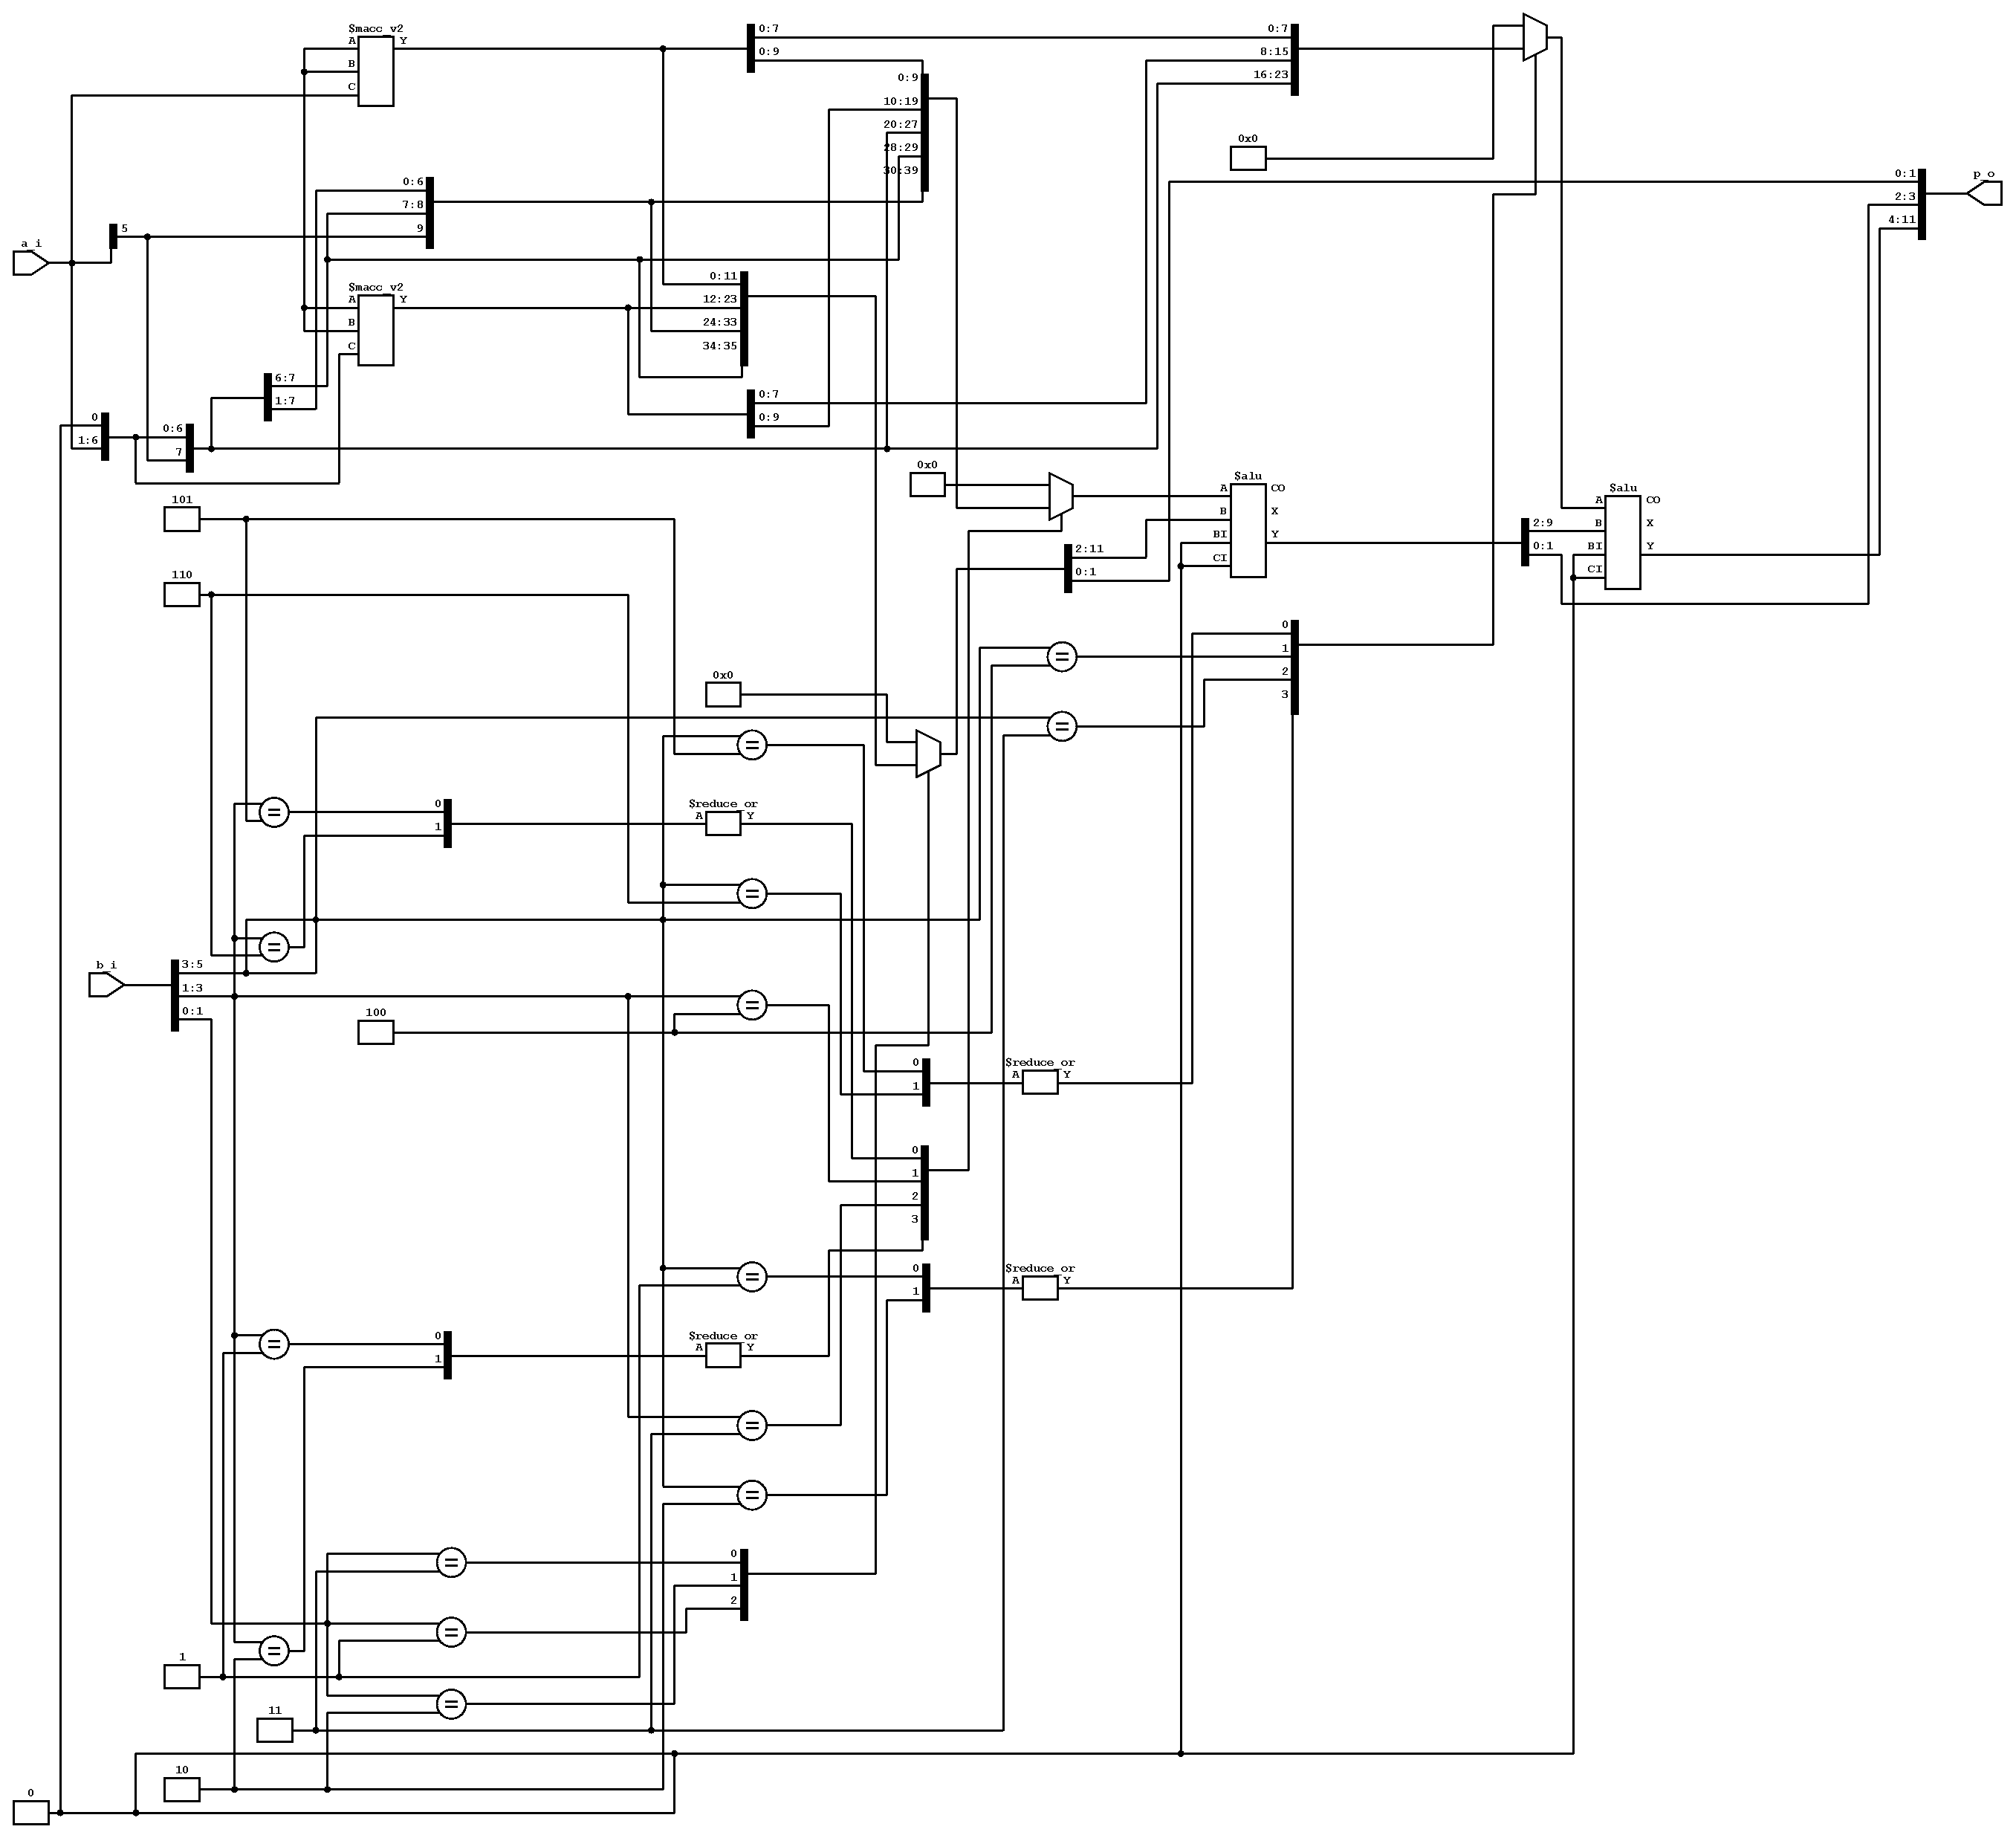
\includegraphics[width=0.92\linewidth]{figures/sch_booth_w6.pdf}
  \caption{Yosys RTL schematic of \code{booth\_multiplier} with $W=6$
    (word-level cells: \code{\$eq} group decoders, Booth-recoding \code{\$pmux}, partial-product \code{\$macc}/\code{\$alu}).}
  \label{fig:sch_booth}
\end{figure}

\begin{figure}[H]
  \centering
  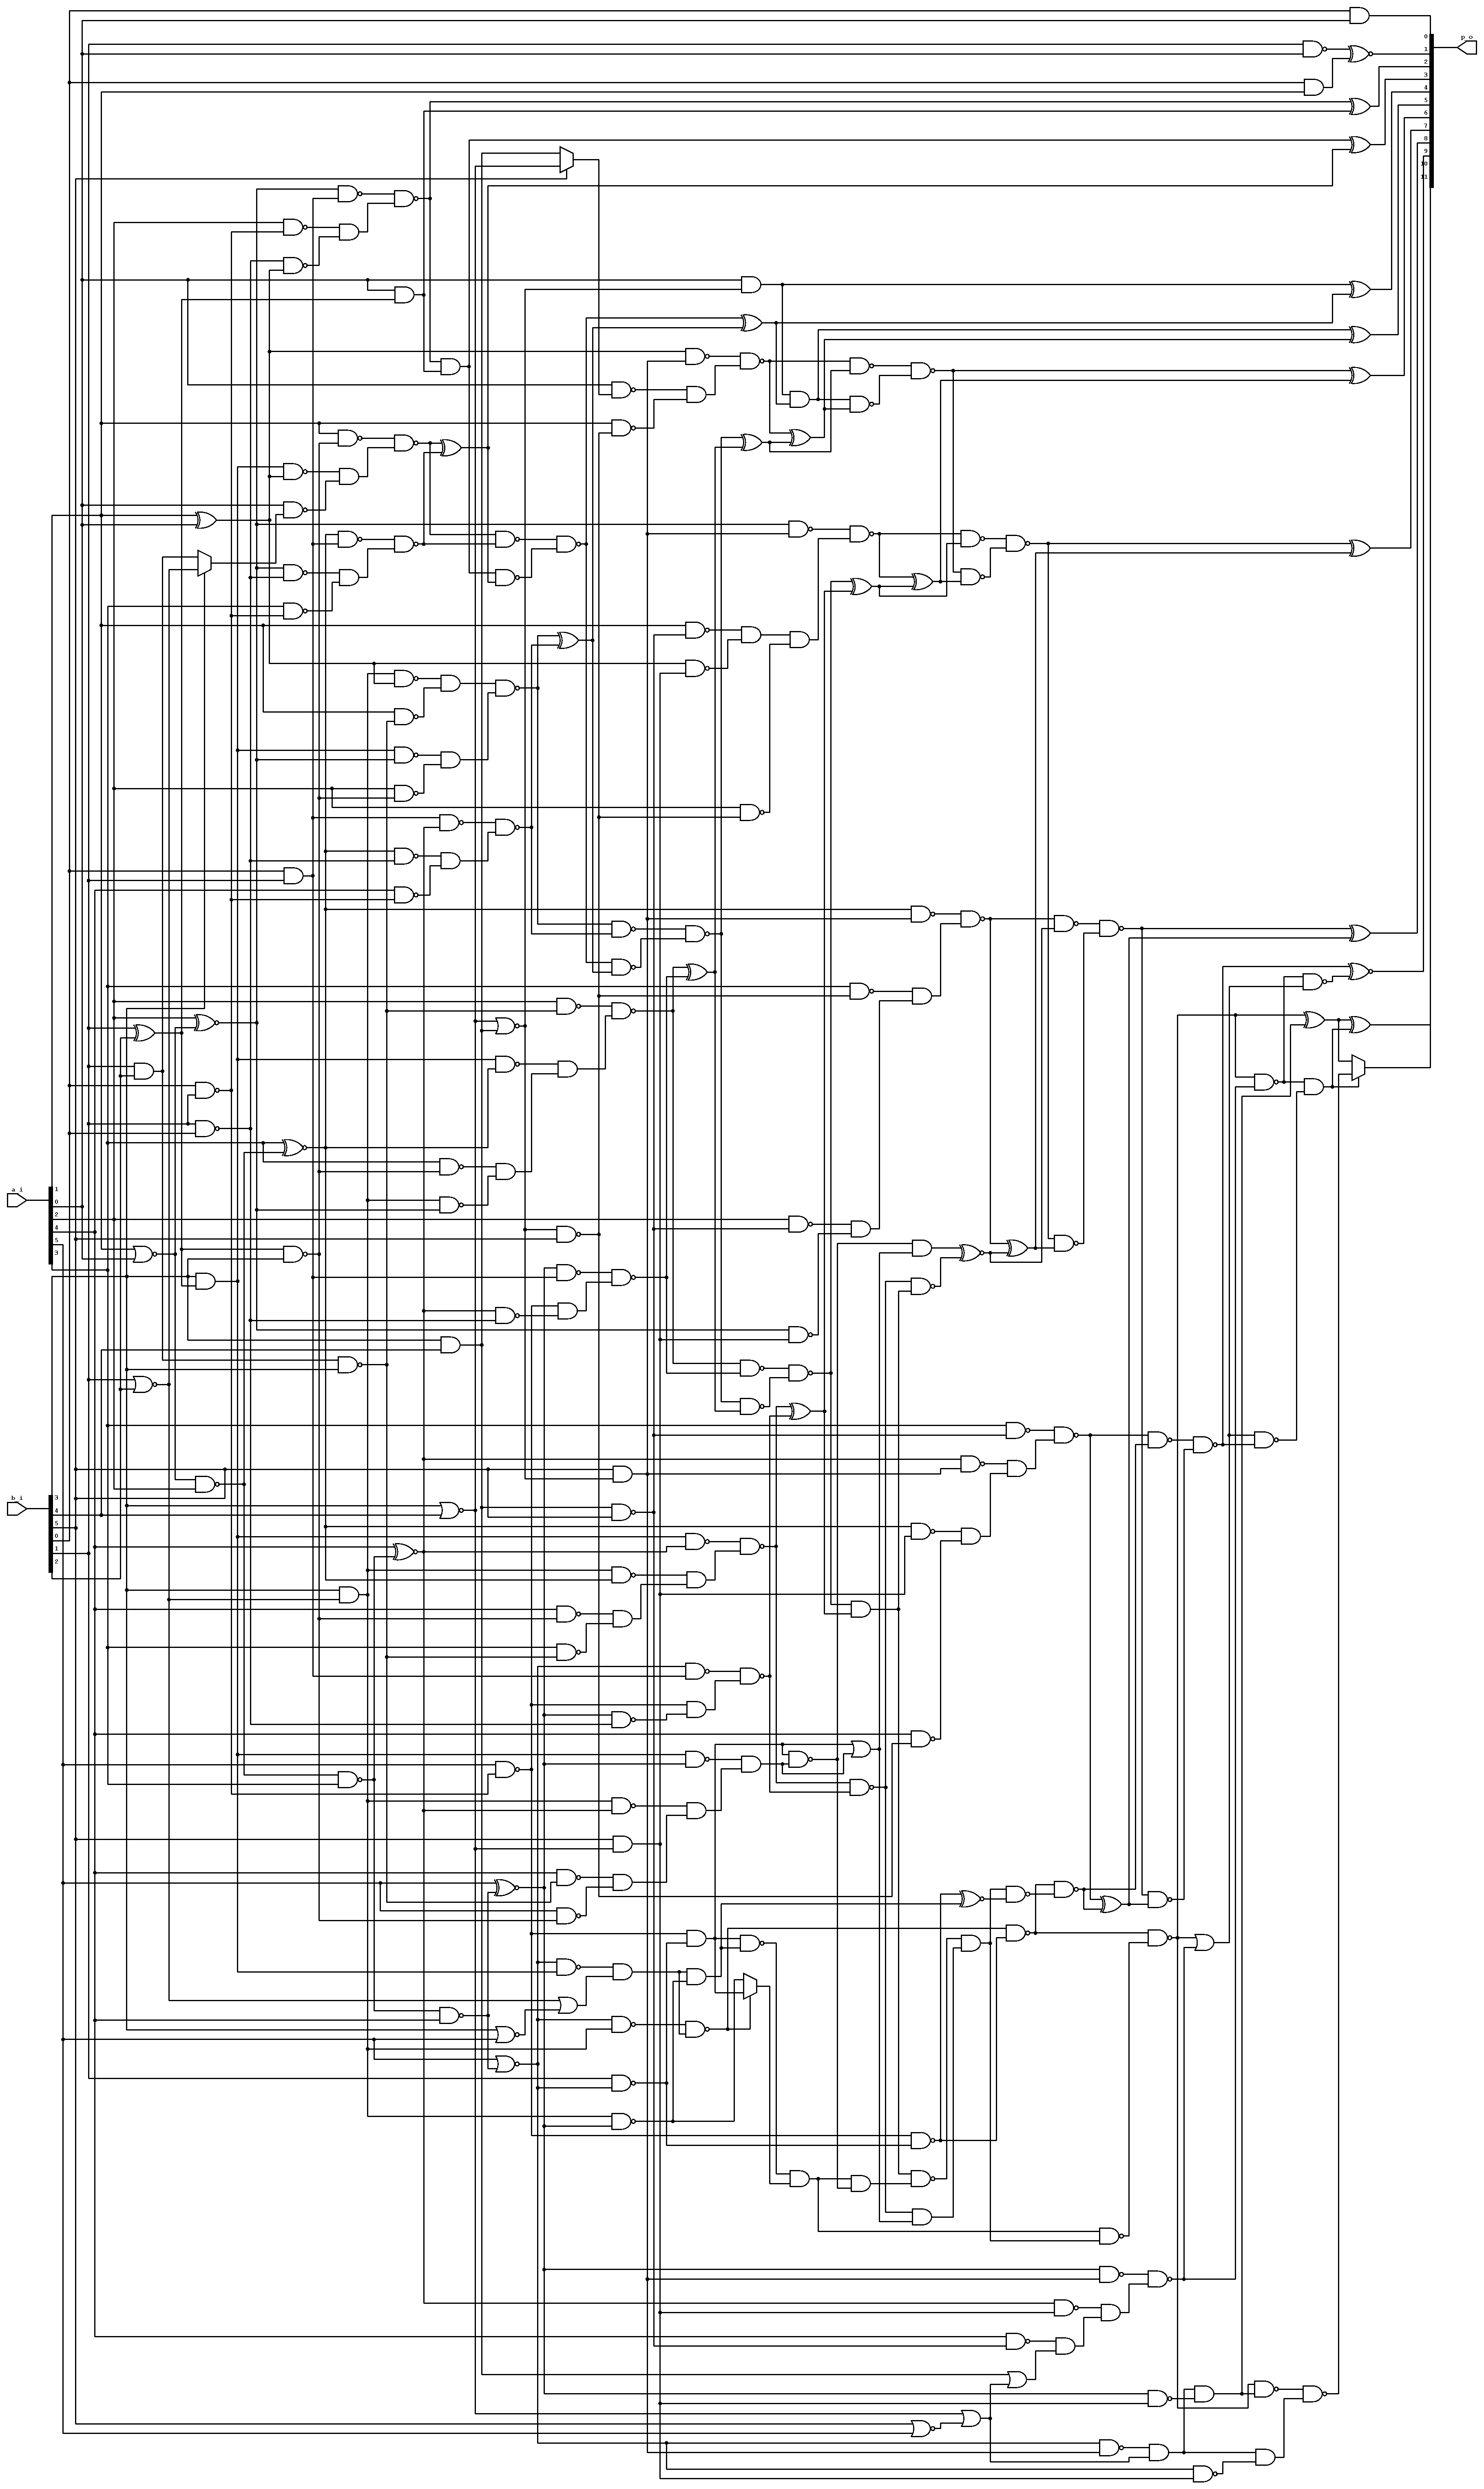
\includegraphics[height=0.80\textheight]{figures/sch_booth_w6_gates.pdf}
  \caption{The same 6-bit Booth multiplier after gate-level synthesis (216 gates).}
  \label{fig:sch_booth_g}
\end{figure}

\begin{figure}[p]
  \centering
  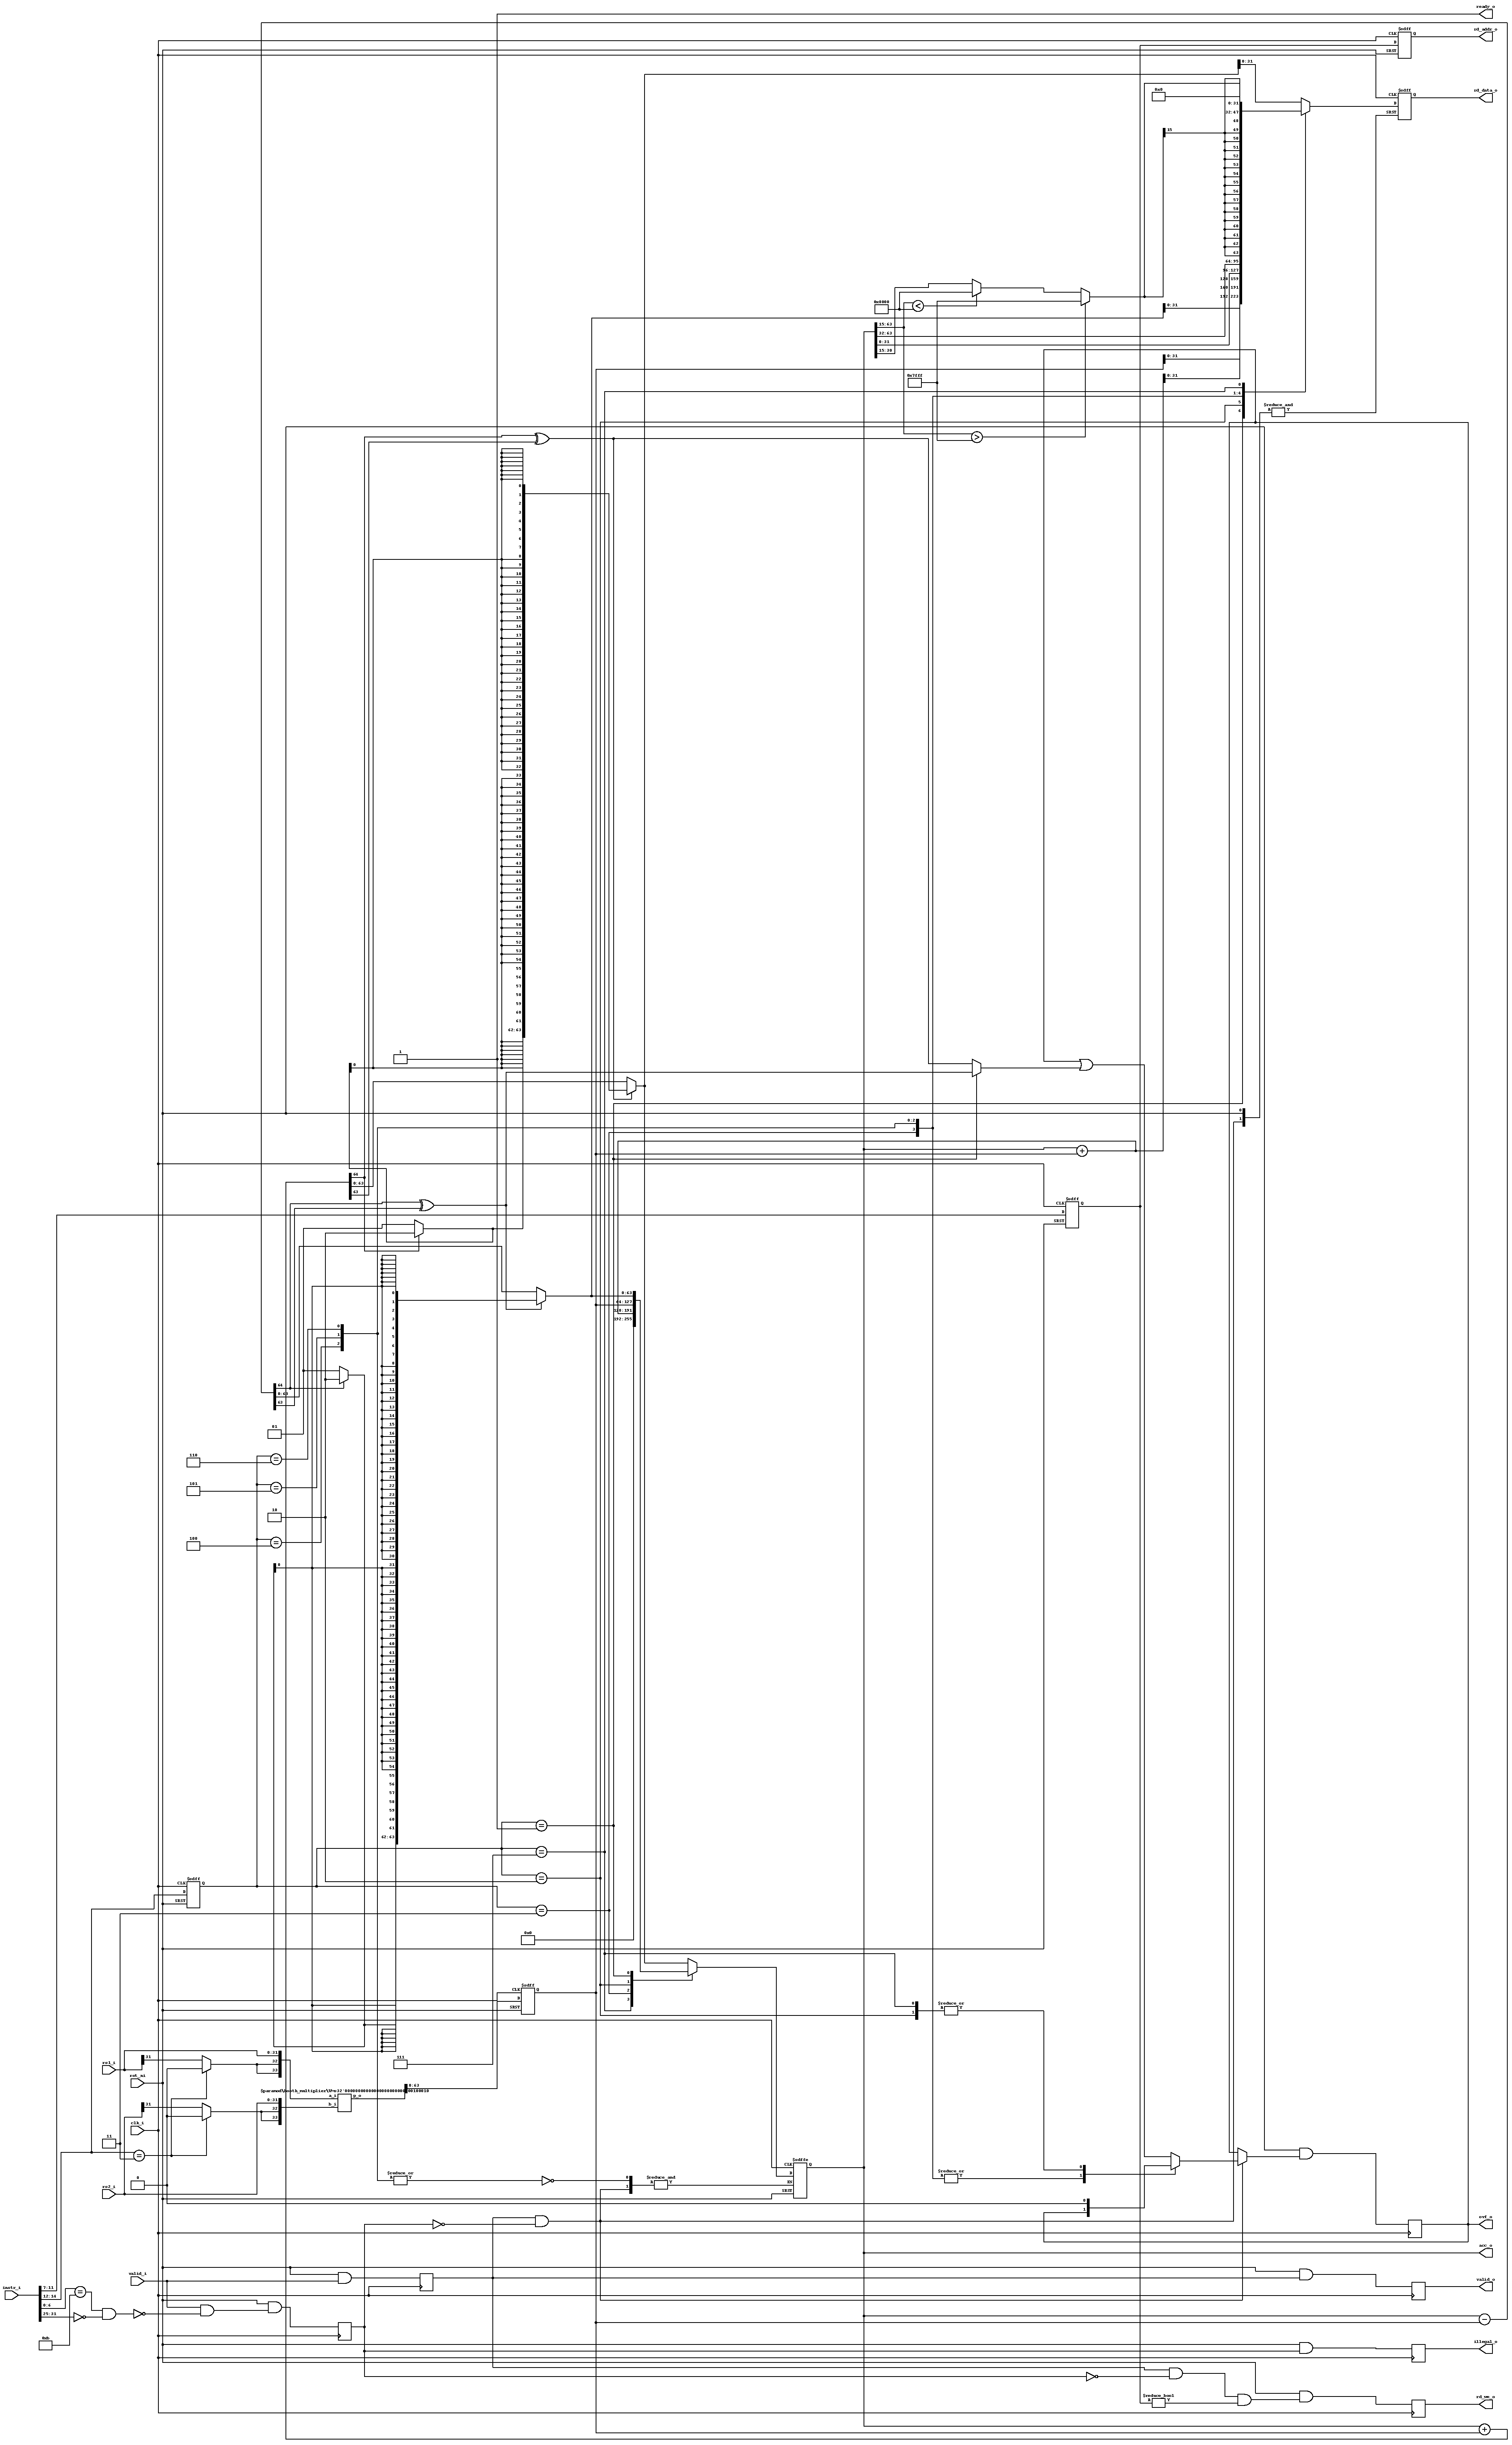
\includegraphics[height=0.86\textheight]{figures/sch_mac_unit.pdf}
  \caption{Yosys RTL schematic of the complete \code{mac\_unit} (Booth
    multiplier shown as a single block).}
  \label{fig:sch_mac}
\end{figure}

\section{Generic gate-level synthesis of the MAC unit}
The flow \code{synth -flatten} followed by
\code{abc -g AND,NAND,OR,NOR,XOR,XNOR,ANDNOT,ORNOT,MUX} produces the netlist
summarised in Table~\ref{tab:gen} and Figure~\ref{fig:syncells}.
\code{check -assert} reports no combinational loops, no multiple drivers,
no undriven nets and no inferred latches.

\begin{table}[H]
  \centering
  \caption{Generic synthesis result (flattened \code{mac\_unit}).}
  \label{tab:gen}
  \small
  \begin{tabular}{@{}lr@{\qquad}lr@{}}
    \toprule
    Cell type & Count & Cell type & Count \\
    \midrule
    NAND   & 5027 & NOT    & 74 \\
    AND    & 1785 & MUX    & 32 \\
    XOR    & 1459 & DFF, sync.\ reset (\code{\$\_SDFF\_})         & 114 \\
    OR     & 376  & DFF, sync.\ reset + enable (\code{\$\_SDFFE\_}) & 65 \\
    NOR    & 226  & \textbf{Total cells} & \textbf{9532} \\
    XNOR   & 199  & \textbf{Flip-flops} & \textbf{179} \\
    ANDNOT / ORNOT & 96 / 79 & Est.\ transistors (\code{stat -tech cmos}) & $\approx$55{,}456 \\
    \bottomrule
  \end{tabular}
\end{table}

\begin{figure}[H]
  \centering
  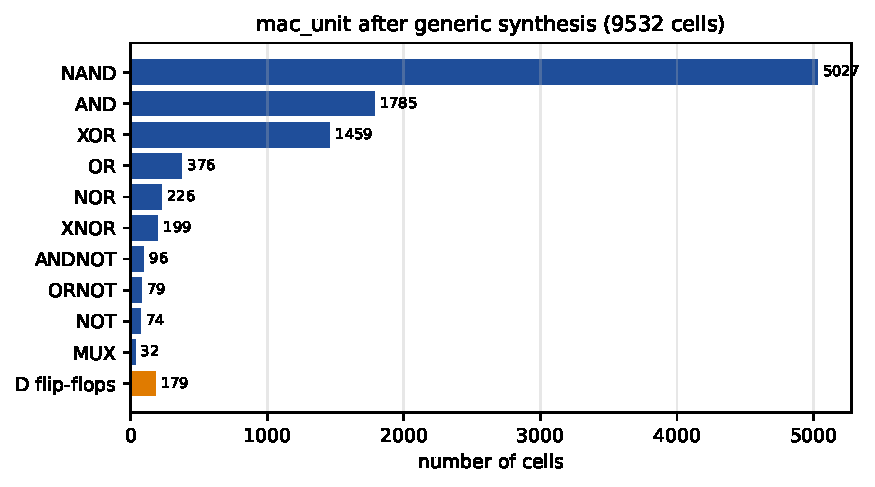
\includegraphics[width=0.75\linewidth]{figures/syn_cells.pdf}
  \caption{Cell-type distribution of the synthesised MAC unit.}
  \label{fig:syncells}
\end{figure}

\paragraph{Register count check.}
The 179 flip-flops match the RTL exactly. Stage~1 holds $1+1+3+5+64=74$ bits
(valid, illegal, \code{funct3}, \code{rd}, product), while stage~2 holds
$64+1+1+5+1+32+1=105$ bits (ACC, OVF, valid, \code{rd}, write enable, data,
illegal). The 65 flip-flops with an enable input are the accumulator and the
OVF flag.
They keep their value on read-only instructions; Yosys inferred the enable
from the default assignment \code{acc\_nxt = acc\_q}.

\paragraph{Logic depth.}
The longest combinational path (\code{ltp}) is \textbf{127 gate levels}, from
the operands through the multiplier to \code{s1\_prod[63]}. For comparison,
the Booth module was replaced by \code{*} and synthesised with Yosys' own
Booth-encoder + Wallace-tree generator (\code{synth -booth}). That version uses
21\,\% fewer gates (7{,}541) but its depth is the same (128 levels). In both
cases, the depth comes from the ripple-carry carry-propagate adders, which
account for about two gate levels per bit, not from the partial-product
reduction.

\section{Area breakdown: MAC unit and complete processor}
Figure~\ref{fig:synarea} compares the hierarchical gate counts. In the
stand-alone MAC unit, the Booth multiplier accounts for 79\,\% of the logic
(7{,}852 of 9{,}990 cells). The complete processor, synthesised by the
script \code{synth/synth\_core.ys}, contains 25{,}286 gates in total. Of these, the
RV32 pipeline makes up 15{,}303, which includes the register file implemented
as 1{,}024 flip-flops (the generic flow has no RAM cells) together with the
RV32M 33$\times$33 multiplier; the MAC unit's control and accumulator take
2{,}138 gates; and the Booth multiplier takes 7{,}845 gates. Adding the full
DSP extension therefore costs about 40\,\% of the processor's gate count.

\begin{figure}[H]
  \centering
  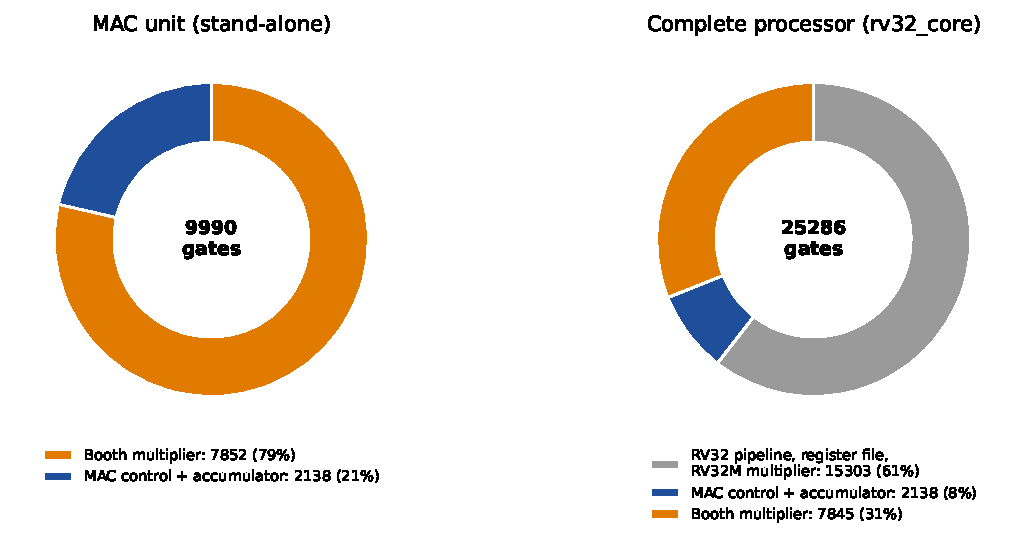
\includegraphics[width=\linewidth]{figures/syn_area.pdf}
  \caption{Generic-gate area breakdown of the MAC unit and of the complete processor.}
  \label{fig:synarea}
\end{figure}

\section{FPGA implementation on the Lattice ECP5}
Three designs were placed and routed. Design~A is the MAC unit with the Booth
multiplier, in which the radix-4 Booth multiplier is built from LUTs and carry
chains. Design~B is the MAC unit with DSP multipliers: the Booth module is
replaced by \code{synth/native\_multiplier.v} (\code{*}), so the
multiplication maps onto four hard \code{MULT18X18D} blocks, and it serves as
a comparison point only. Design~C is the complete processor, \code{rv32\_core}
including the MAC unit with the Booth multiplier; here the register file maps
to 32 LUT-RAM blocks and the RV32M multiplier to DSP blocks, while the
instruction and data memories are outside the core.
For A and B, the unit is wrapped in \code{synth/fmax\_wrapper.v}, which
registers every input and output, so that every timing path is
register-to-register, as it would be inside a processor.

\begin{table}[H]
  \centering
  \caption{ECP5 LFE5U-85F implementation results (post place \& route).}
  \label{tab:ecp5}
  \small
  \begin{tabular}{@{}lrrr@{}}
    \toprule
    Metric & A: MAC (Booth) & B: MAC (DSP) & C: RV32IM core + MAC \\
    \midrule
    LUT4 (Yosys)                     & 5{,}108 & 611 & 6{,}486 \\
    PFUMX / L6MUX21 (wide muxes)     & 1{,}855 / 584 & 210 / 52 & 1{,}992 / 631 \\
    CCU2C (carry cells)              & 155 & 162 & 399 \\
    Flip-flops (design)              & 179 & 179 & 730 \\
    LUT-RAM blocks (DPR16X4)         & 0 & 0 & 32 \\
    MULT18X18D (DSP multipliers)     & 0 & 4 & 4 \\
    Logic cells after P\&R           & 4{,}854 (5.8\,\%) & 963 (1.2\,\%) & 7{,}566 (9.0\,\%) \\
    I/O pins                         & 204 & 204 & 330 \\
    \midrule
    Critical path (reg $\rightarrow$ reg) & 17.73\,ns & 12.69\,ns & 28.94\,ns \\
    \quad of which logic / routing   & 6.0 / 11.8\,ns & 7.9 / 4.8\,ns & 10.1 / 18.9\,ns \\
    \textbf{Maximum frequency $F_{\max}$} & \textbf{56.4\,MHz} & \textbf{78.8\,MHz} & \textbf{34.6\,MHz} \\
    \bottomrule
  \end{tabular}
\end{table}

\begin{figure}[H]
  \centering
  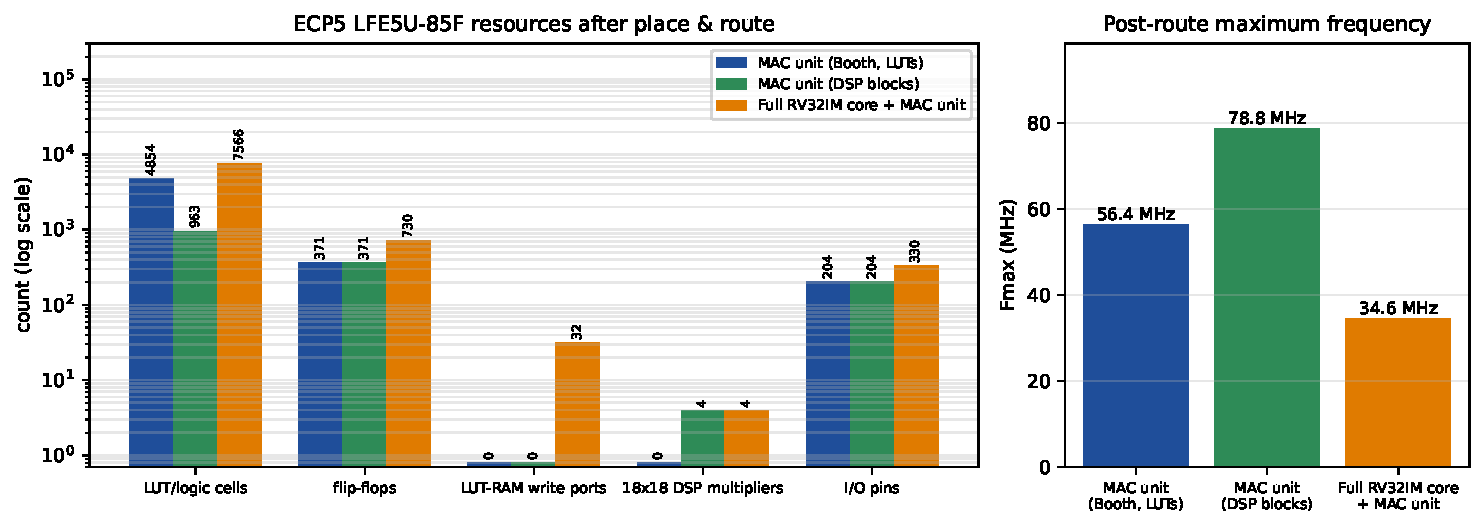
\includegraphics[width=\linewidth]{figures/fpga_resources.pdf}
  \caption{ECP5 resource usage (log scale) and post-route $F_{\max}$ of the three designs.}
  \label{fig:fpgares}
\end{figure}

\paragraph{Critical paths.}
Figure~\ref{fig:critpath} plots the cumulative delay along each design's
critical path, as reported by nextpnr. For designs A and B, the path starts at
the input operand register, passes through the stage-1 multiplier and ends at
the \code{s1\_prod} pipeline register; the stage-2 accumulate path is shorter,
which confirms that the MAC pipeline is split in the right place. In the Booth
version, routing (11.8\,ns) dominates logic (6.0\,ns), because the LUT-based
multiplier is spread over a large area. For the complete processor, the
critical path runs from the WB forwarding control, through the forwarding
multiplexer and the \emph{single-cycle RV32M multiplier} (DSP blocks plus
carry-chain adders), to the EX/MEM result register, so in the full CPU it is
the baseline \code{mul} instruction, not the pipelined MAC unit, that limits
the clock.

\begin{figure}[H]
  \centering
  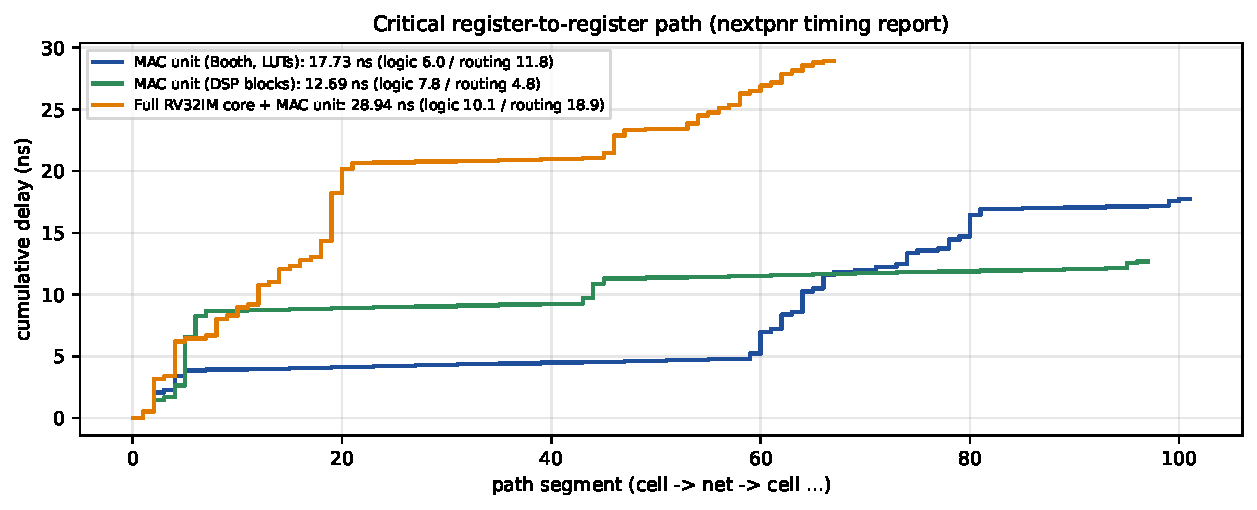
\includegraphics[width=\linewidth]{figures/fpga_critpath.pdf}
  \caption{Cumulative delay along the critical register-to-register path of each design.}
  \label{fig:critpath}
\end{figure}

\begin{figure}[H]
  \centering
  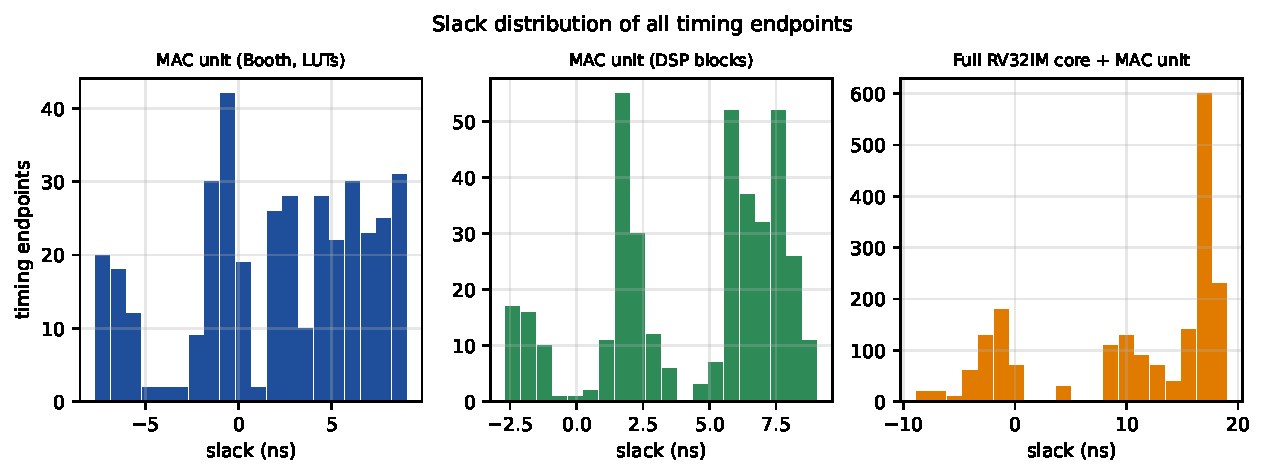
\includegraphics[width=\linewidth]{figures/fpga_slack.pdf}
  \caption{Slack histograms of all timing endpoints (100\,MHz target for A/B, 50\,MHz for C).}
  \label{fig:slack}
\end{figure}

\paragraph{Floorplans.}
Figures~\ref{fig:fp_mac} and~\ref{fig:fp_core} are die renders of the
placed-and-routed designs, drawn from nextpnr's output
(\code{report/scripts/export\_floorplan.py}). Each square is one programmable
tile of the ECP5 die (tile coordinates X\,0--126, Y\,0--95), coloured by the
block whose cells nextpnr placed there; brighter means more cells in the tile.
The copper glow underneath is the routing density (routed wire segments per
tile, log scale), the ring of small squares is the used I/O pads, and the
white line is the critical path, from its start (dot) to its end (star). An
interactive version, with zoom, per-block highlighting and a per-tile
breakdown, is on the project page. The Booth multiplier (orange) forms one
dense block, with the MAC stage-2 logic (blue) at its edge, and it is the
routing hot spot. In the complete processor, the core logic, the MAC unit and
the four DSP blocks are packed into one region in the upper-left corner, close
to the I/O pins on the top edge.

\begin{figure}[H]
  \centering
  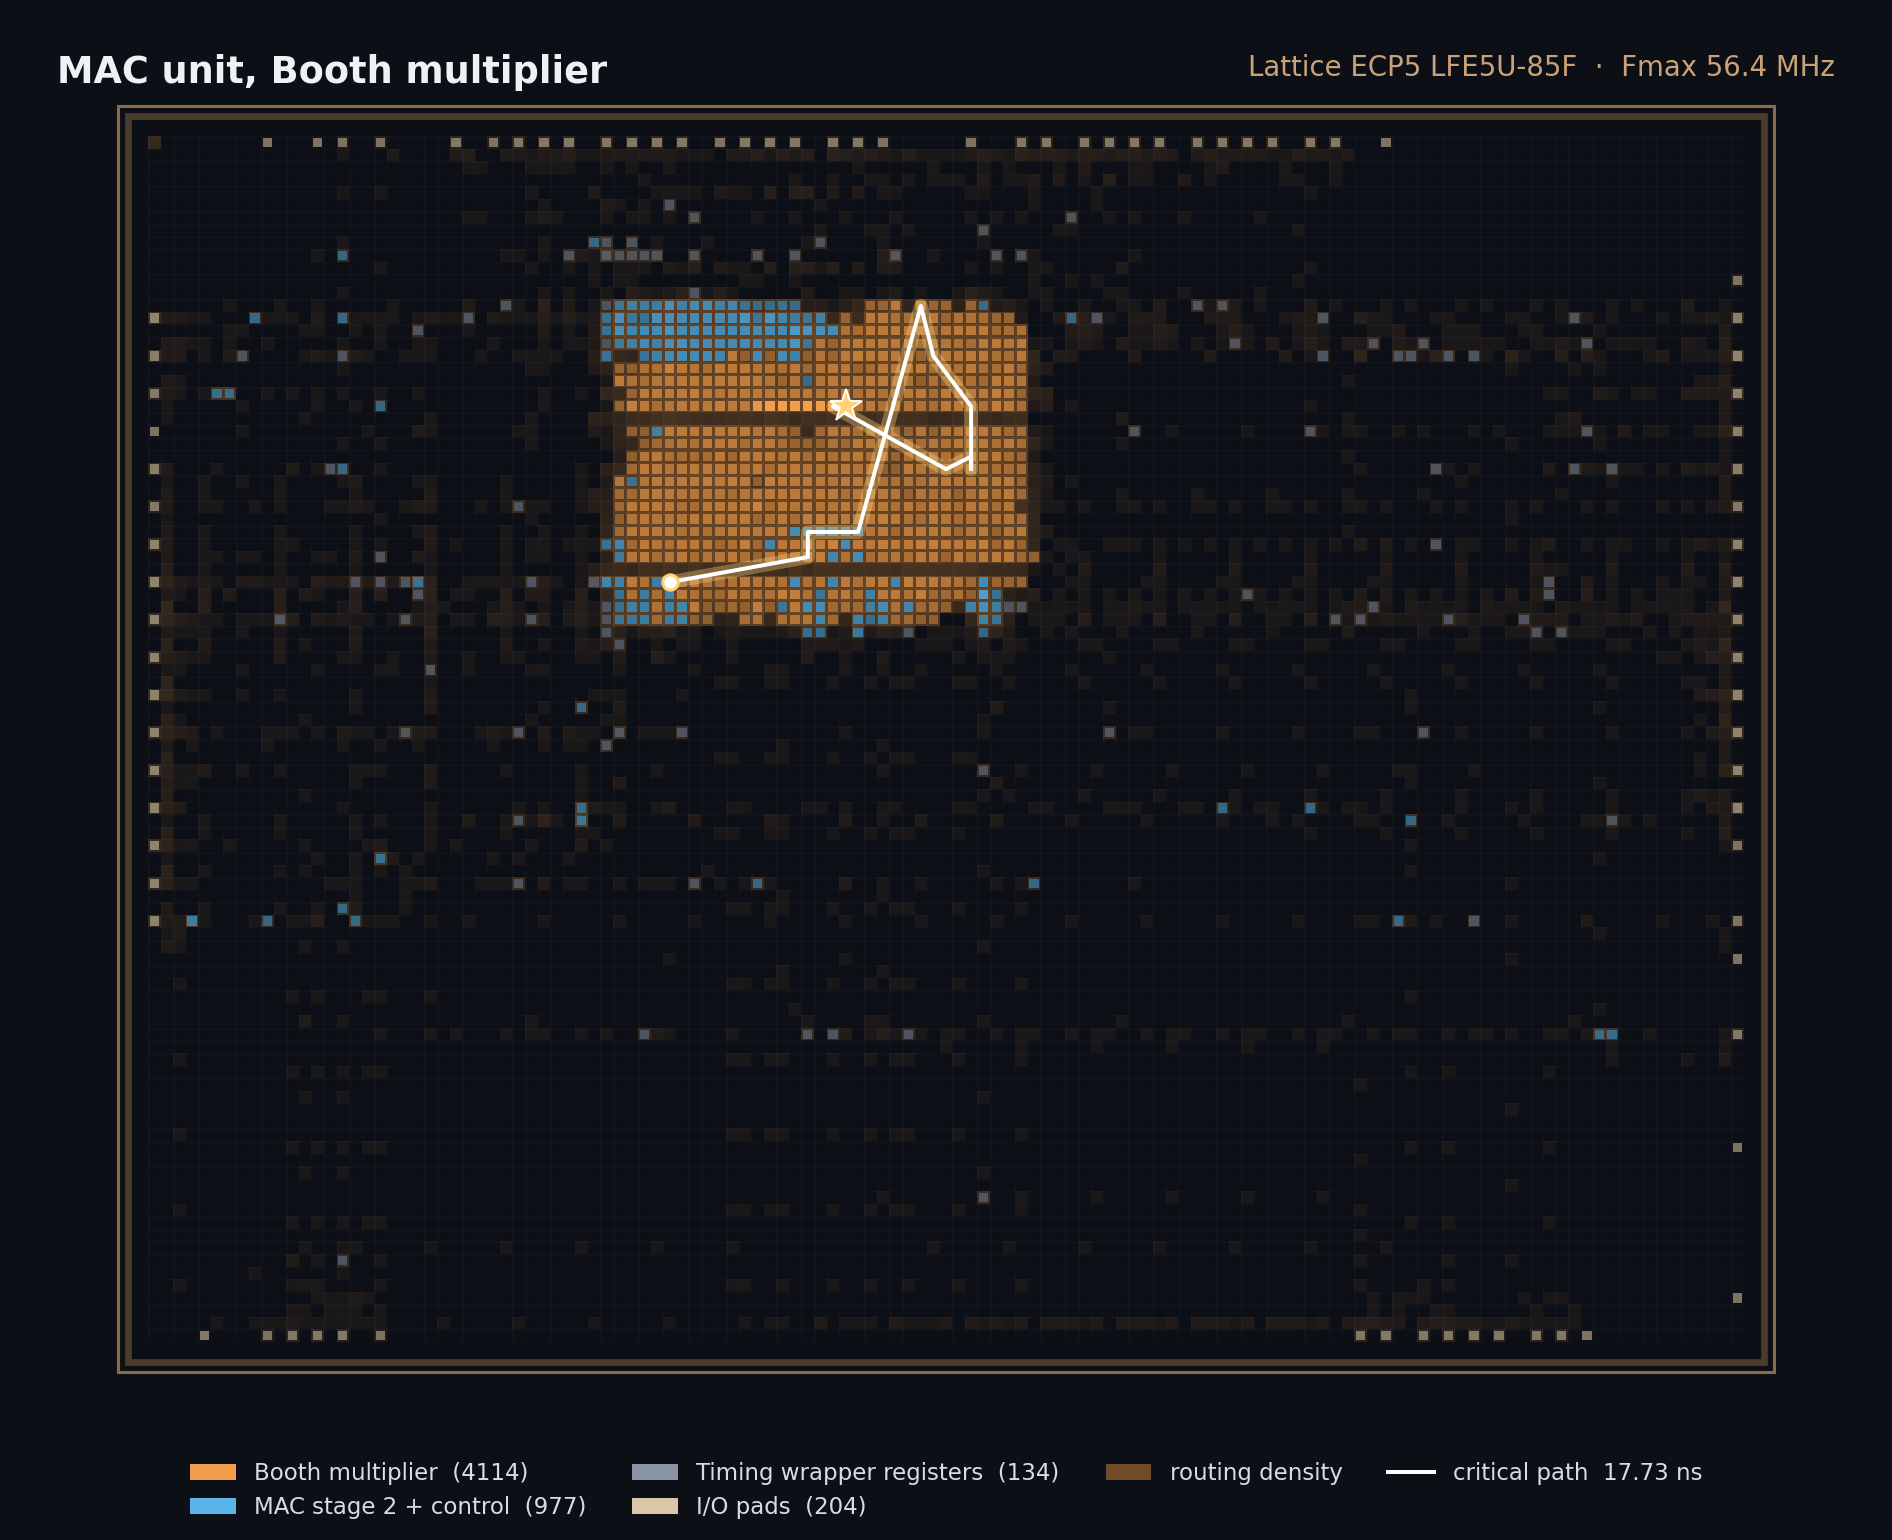
\includegraphics[width=0.92\linewidth]{figures/floorplan_mac.png}
  \caption{Die render of the MAC unit (design A) on the ECP5: placement by
    block, routing density and critical path.}
  \label{fig:fp_mac}
\end{figure}

\begin{figure}[H]
  \centering
  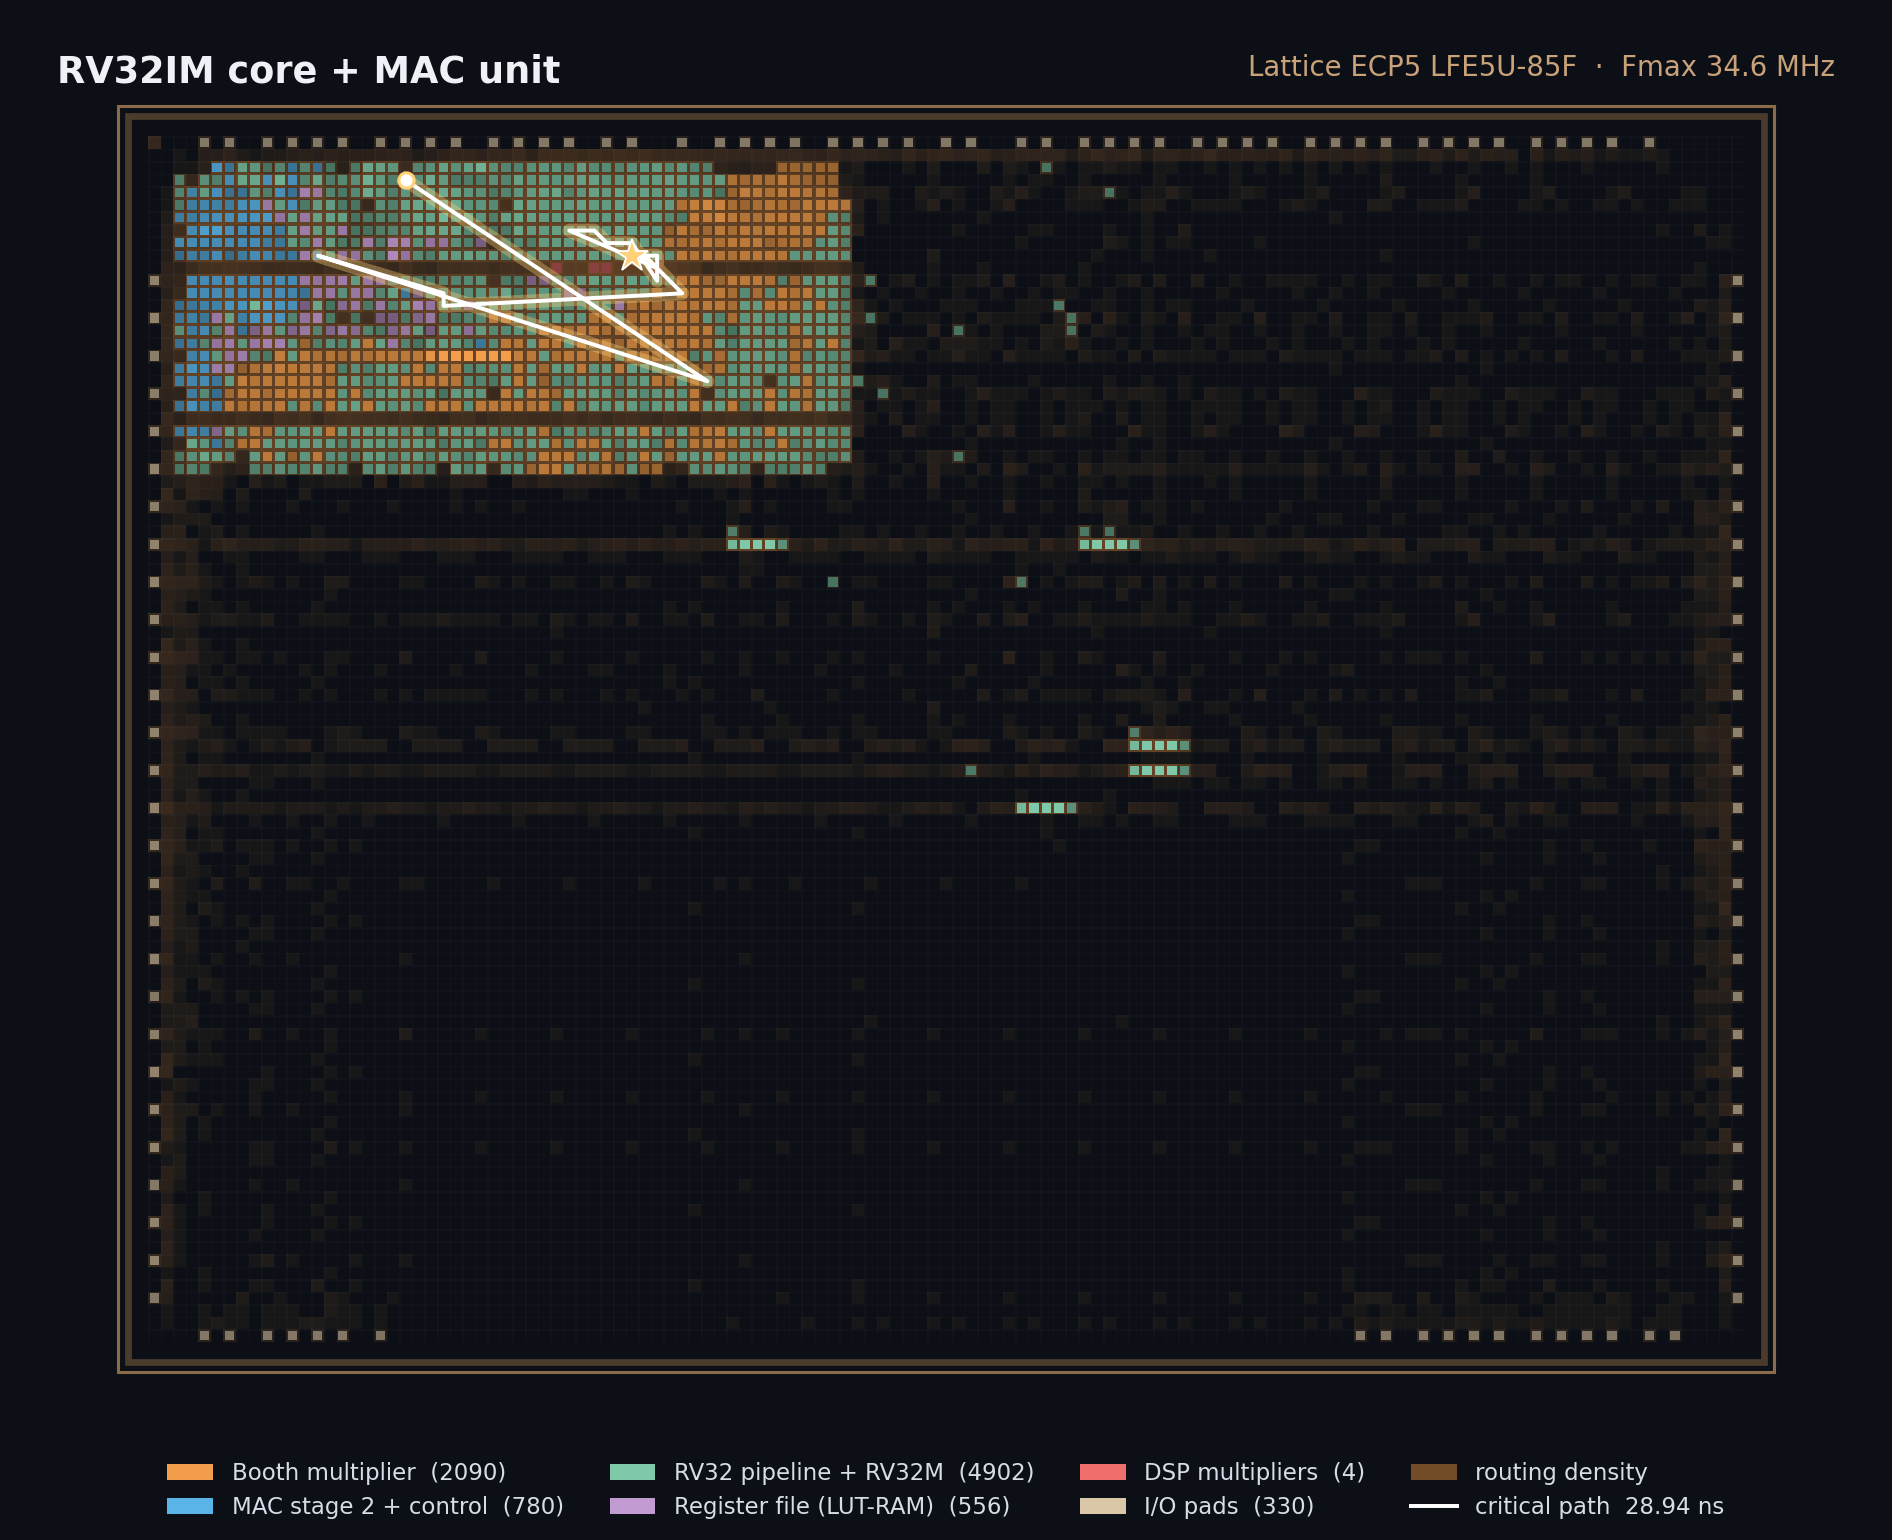
\includegraphics[width=0.92\linewidth]{figures/floorplan_core.png}
  \caption{Die render of the complete RV32IM core with the MAC unit (design C).
    The register file (purple) sits next to the MAC unit; the critical path
    runs through the RV32M multiplier on the DSP blocks.}
  \label{fig:fp_core}
\end{figure}

\paragraph{Interpretation.}
On an FPGA, the hand-written Booth multiplier uses about 8$\times$ more LUTs
than the DSP version and is 28\,\% slower. This is expected, because FPGAs
contain hard multipliers. The Booth design is still the right choice for this
project: it shows the algorithm explicitly, it is fully portable, and it is
what an ASIC implementation would use. For an FPGA product, variant~B would
be preferred.

\section{Post-synthesis gate-level simulation}
The flattened gate-level netlist written by Yosys
(\code{synth/out/mac\_unit\_netlist.v}, about 19{,}000 lines) was simulated with
the \emph{unchanged} testbench \code{tb\_mac\_unit.v}. It passed all tests
(Listing~\ref{lst:gate}). This confirms that synthesis preserved the
behaviour of the RTL and that there are no simulation/synthesis mismatches.
The gate-level simulation has zero delay, so it checks function only; timing
is covered by the static timing analysis above.

\begin{lstlisting}[style=log, caption={Gate-level simulation result (\code{sim/gate/mac\_gate\_sim.log}).}, label={lst:gate}]
 FUNCTIONAL COVERAGE
   mac=570 msu=338 mul.acc=378 macu=381 rdacc.lo=346 rdacc.hi=386 rdacc.q15=393 clracc=374
   illegal=162  saturation events=7  rd=x0 writes=360  bubble gaps=684
 RESULTS
   instructions issued : 3328
   checks performed    : 3351
   errors              : 0
   >>> ALL TESTS PASSED <<<
\end{lstlisting}
